\documentclass[../../LearnCpp.tex]{subfiles}

\begin{document}

\asubsection{9}{Multiple inheritance}

C++ 提供了多重继承的能力。\textbf{多重继承} multiple inheritance让派生类从若干父类中继承成员。

\begin{figure}[ht]
    \centering
    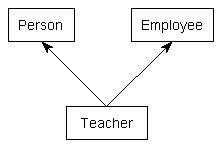
\includegraphics[width=5cm]{\subfix{../images/PersonTeacher}}

    \label{fig:PersonTeacher}
    \caption{PersonTeacher}
\end{figure}

\begin{lstlisting}[language=C++]
#include <string>
#include <string_view>

class Person
{
  private:
  std::string m_name;
  int m_age{};

  public:
  Person(std::string_view name, int age)
      : m_name{name}, m_age{age}
  {
  }

  const std::string& getName() const { return m_name; }
  int getAge() const { return m_age; }
};

class Employee
{
  private:
  std::string m_employer;
  double m_wage{};

  public:
  Employee(std::string_view employer, double wage)
      : m_employer{employer}, m_wage{wage}
  {
  }

  const std::string& getEmployer() const { return m_employer; }
  double getWage() const { return m_wage; }
};

// Teacher 公共继承 Person 与 Employee
class Teacher : public Person, public Employee
{
  private:
  int m_teachesGrade{};

  public:
  Teacher(std::string_view name, int age, std::string_view employer,
          double wage, int teachesGrade)
      : Person{name, age}, Employee{employer, wage}, m_teachesGrade{teachesGrade}
  {
  }
};
\end{lstlisting}

\subsubsection*{Mixins}

\textbf{mixin} 是一种为了给类添加属性的,且用作于继承的小型类。
mixin 这个名字意味着类的作用是混合进其它类,而不自己进行实例化。

下面代码中,\acode{Box} 与 \acode{Label} 类作为 mixins 用于继承并创建新的 \acode{Button} 类。

\begin{lstlisting}[language=C++]
#include <string>

struct Point2D
{
  int x;
  int y;
};

class Box
{
  private:
  Point2D m_topLeft{};
  Point2D m_bottomRight{};

  public:
  void setTopLeft(Point2D point) { m_topLeft = point; }
  void setBottomRight(Point2D point) { m_bottomRight = point; }
};

class Label
{
  private:
  std::string m_text{};
  int m_fontSize{};

  public:
  void setText(const std::string_view str) { m_text = str; }
  void setFontSize(int fontSize) { m_fontSize = fontSize; }
};

class Button : public Box, public Label
{
};
\end{lstlisting}

\subsubsection*{进阶}

因为 mixins 是设计来给派生类添加功能,而不是提供接口,mixins 通常不使用虚函数(下一章节覆盖)。
相反的是,如果 mixin 类需要自定义特俗用途,则通常使用模版。正因如此,mixin 类多为模版化的。

使用派生类为模版类型参数,传递给自己的基类。
这样的继承被称为 \textbf{Curiously Recurring Template Pattern}(简称 CRTP),类似如下:

\begin{lstlisting}[language=C++]
// The Curiously Recurring Template Pattern (CRTP)

template <class T>
class Mixin
{
    // Mixin<T> can use template type parameter T to access members of Derived
    // via (static_cast<T*>(this))
};

class Derived : public Mixin<Derived>
{
};
\end{lstlisting}

\subsubsection*{多重继承的问题}

由于多重继承看起来像是单个继承的拓展,
多重继承引入了很多问题可以显著的增加程序的复杂性,同时使得它们的维护变成噩梦。
现在来看一些这样的情况。

首先,可能会出现模棱两可的情况,当若干基类包含同名函数。

\begin{lstlisting}[language=C++]
#include <iostream>

class USBDevice
{
private:
    long m_id {};

public:
    USBDevice(long id)
        : m_id { id }
    {
    }

    long getID() const { return m_id; }
};

class NetworkDevice
{
private:
    long m_id {};

public:
    NetworkDevice(long id)
        : m_id { id }
    {
    }

    long getID() const { return m_id; }
};

class WirelessAdapter: public USBDevice, public NetworkDevice
{
public:
    WirelessAdapter(long usbId, long networkId)
        : USBDevice { usbId }, NetworkDevice { networkId }
    {
    }
};

int main()
{
    WirelessAdapter c54G { 5442, 181742 };
    std::cout << c54G.getID(); // 哪个 getID() 被调用了?

    return 0;
}
\end{lstlisting}

不过有一种方法可以绕过这个问题:显式指定调用的版本:

\begin{lstlisting}[language=C++]
int main()
{
    WirelessAdapter c54G { 5442, 181742 };
    std::cout << c54G.USBDevice::getID();

    return 0;
}
\end{lstlisting}

其次,一个更严肃的问题是菱形问题。

\begin{lstlisting}[language=C++]
class PoweredDevice
{
};

class Scanner: public PoweredDevice
{
};

class Printer: public PoweredDevice
{
};

class Copier: public Scanner, public Printer
{
};
\end{lstlisting}

\begin{figure}[ht]
    \centering
    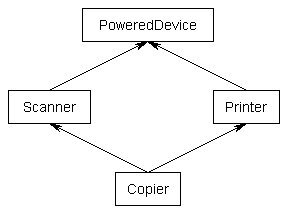
\includegraphics[width=5cm]{\subfix{../images/PoweredDevice}}
    \label{fig:PoweredDevice}
    \caption{PoweredDevice}
\end{figure}

下一章节会讲解如何解决这个问题。

\subsubsection*{多重继承是否值得?}

事实证明,大多数可以使用多重继承来解决的问题也可以被单独继承解决。
很多面向对象语言甚至于不支持多重继承。
很多相关的现代语言如 Java 和 C\# 限制类为单独继承普通类,但是允许多重继承接口类(之后会提到)。
这些语言中的禁止多重继承概念反而使得语言变得更复杂,最终导致更多问题。

最佳实践:避免多重继承,除非不这么做会导致更大的复杂性。

\end{document}
